% La Creación de Valor Compartido (CVC) se concibe como un paradigma estratégico que redefine la función y el propósito de la empresa al integrar, de forma inextricable, la generación de beneficios económicos con la solución de problemáticas sociales y ambientales \cite{porter2006strategy}.\\

% En contraste con enfoques tradicionales como la Responsabilidad Social Empresarial (RSE), que a menudo se implementan de manera reactiva y periférica, la CVC se internaliza en el núcleo del modelo de negocio. Esto permite que los desafíos sociales se transformen en oportunidades de innovación, generando sinergias que potencian la competitividad y la sostenibilidad de la organización. Los fundamentos teóricos de la CVC se sustentan en tres dimensiones estratégicas, las cuales se detallan a continuación:

% \begin{enumerate}
%     \item \textbf{Redefinición de productos y mercados:}  
%     Se orienta al desarrollo de bienes y servicios que atienden necesidades sociales no satisfechas. Este proceso implica identificar nichos de mercado donde la solución de un problema social se traduzca en una ventaja competitiva, generando así un impacto positivo tanto en la sociedad como en la rentabilidad de la empresa.
    
%     \item \textbf{Reconfiguración de la cadena de valor:}  
%     Consiste en optimizar los procesos internos y la relación con los proveedores para reducir externalidades negativas. La integración de prácticas sostenibles en la producción (por ejemplo, la eficiencia energética y la economía circular) no solo mejora la eficiencia operativa, sino que también fortalece la imagen corporativa y reduce costos operativos.
    
%     \item \textbf{Desarrollo de Clusters locales:}  
%     Se enfoca en la inversión en infraestructura, capital humano y redes de colaboración con actores locales. El objetivo es potenciar el desarrollo regional y crear un ecosistema en el que la prosperidad de la empresa esté estrechamente vinculada al bienestar de la comunidad circundante.
% \end{enumerate}

% Estos tres ejes permiten conceptualizar la CVC como una herramienta que no solo genera valor económico, sino que también crea externalidades positivas medibles a través de indicadores como el Social Return on Investment (SROI) \cite{porter2006strategy}. La Figura~\ref{fig:CVC_Modelo} ilustra un modelo conceptual que integra estas dimensiones en el proceso de creación de valor compartido.

% \begin{figure}[h!]
%   \centering
%   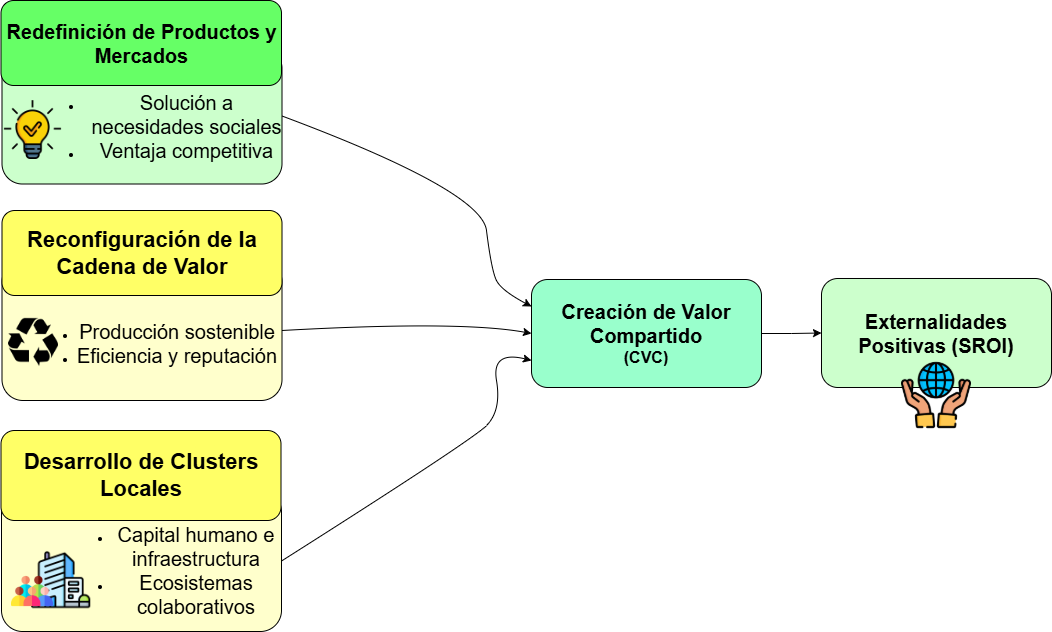
\includegraphics[width=0.65\textwidth]{images/CVC_Modelo.png}
%   \caption{Modelo conceptual de Creación de Valor Compartido (basado de \cite{Por11}).}
%   \label{fig:CVC_Modelo}
% \end{figure}